\section{Components Used}

The components used to build the self-balancing bot and the self-balancing platform are as follows:
\begin{enumerate}
  \item Arduino UNO - 2
  \item MPU6050 Gyroscope - 2
  \item zhengk zytd520 motors - 2
  \item Orange LiPo(4100mAh, 11.1V, 35C) - 1
  \item L298N motor driver - 1
  \item MG995 servo - 1
  \item Mechanix kit - 1
  \item MM Jumper wires
  \item MF Jumper wires
\end{enumerate}

\clearpage

\section{Connections}
\subsection{Self-balancing bot}

\begin{figure}[H]
\centering
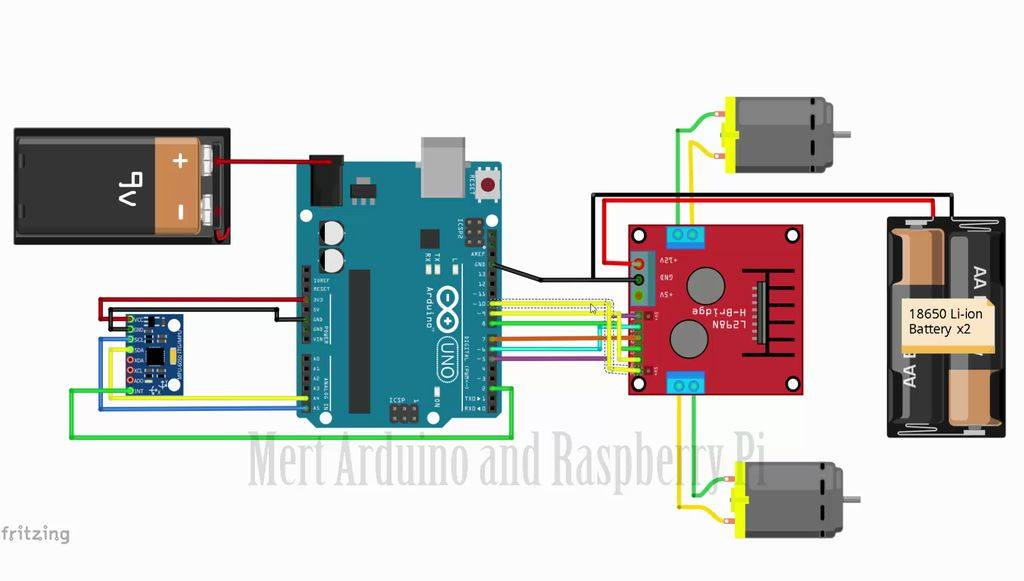
\includegraphics[width=\textwidth,height=\textheight,keepaspectratio]{images/bot-connections}
\caption{Connections for the self-balancing bot}
\label{fig:connections}
\end{figure}

The connections for the self-balancing bot are as depicted in figure \ref{fig:connections}. The Arduino UNO has been powered by connecting the 12V pin from the L298N motor driver to the \textit{Vin} pin on the arduino. The motor driver takes the 12V and GND from the battery and also has additional 5V pins.

\subsection{Self-balancing platform}

For the self-balancing platform, there is another arduino placed at the top of the bot which is connected to an MPU6050 placed on the platfrom. This helps the platform behave as an individual system. The MPU6050 on the platfrom is connected using the same connections for the MPU6050 as shown in figure \ref{fig:connections}. The servo motor is connected to pin number \textit{5} of the arduino. The arduino is powered in the same way the same way as discussed above.

\clearpage

\subsection{Final Connections}

\begin{figure}
\centering
\begin{subfigure}{.5\textwidth}
  \centering
  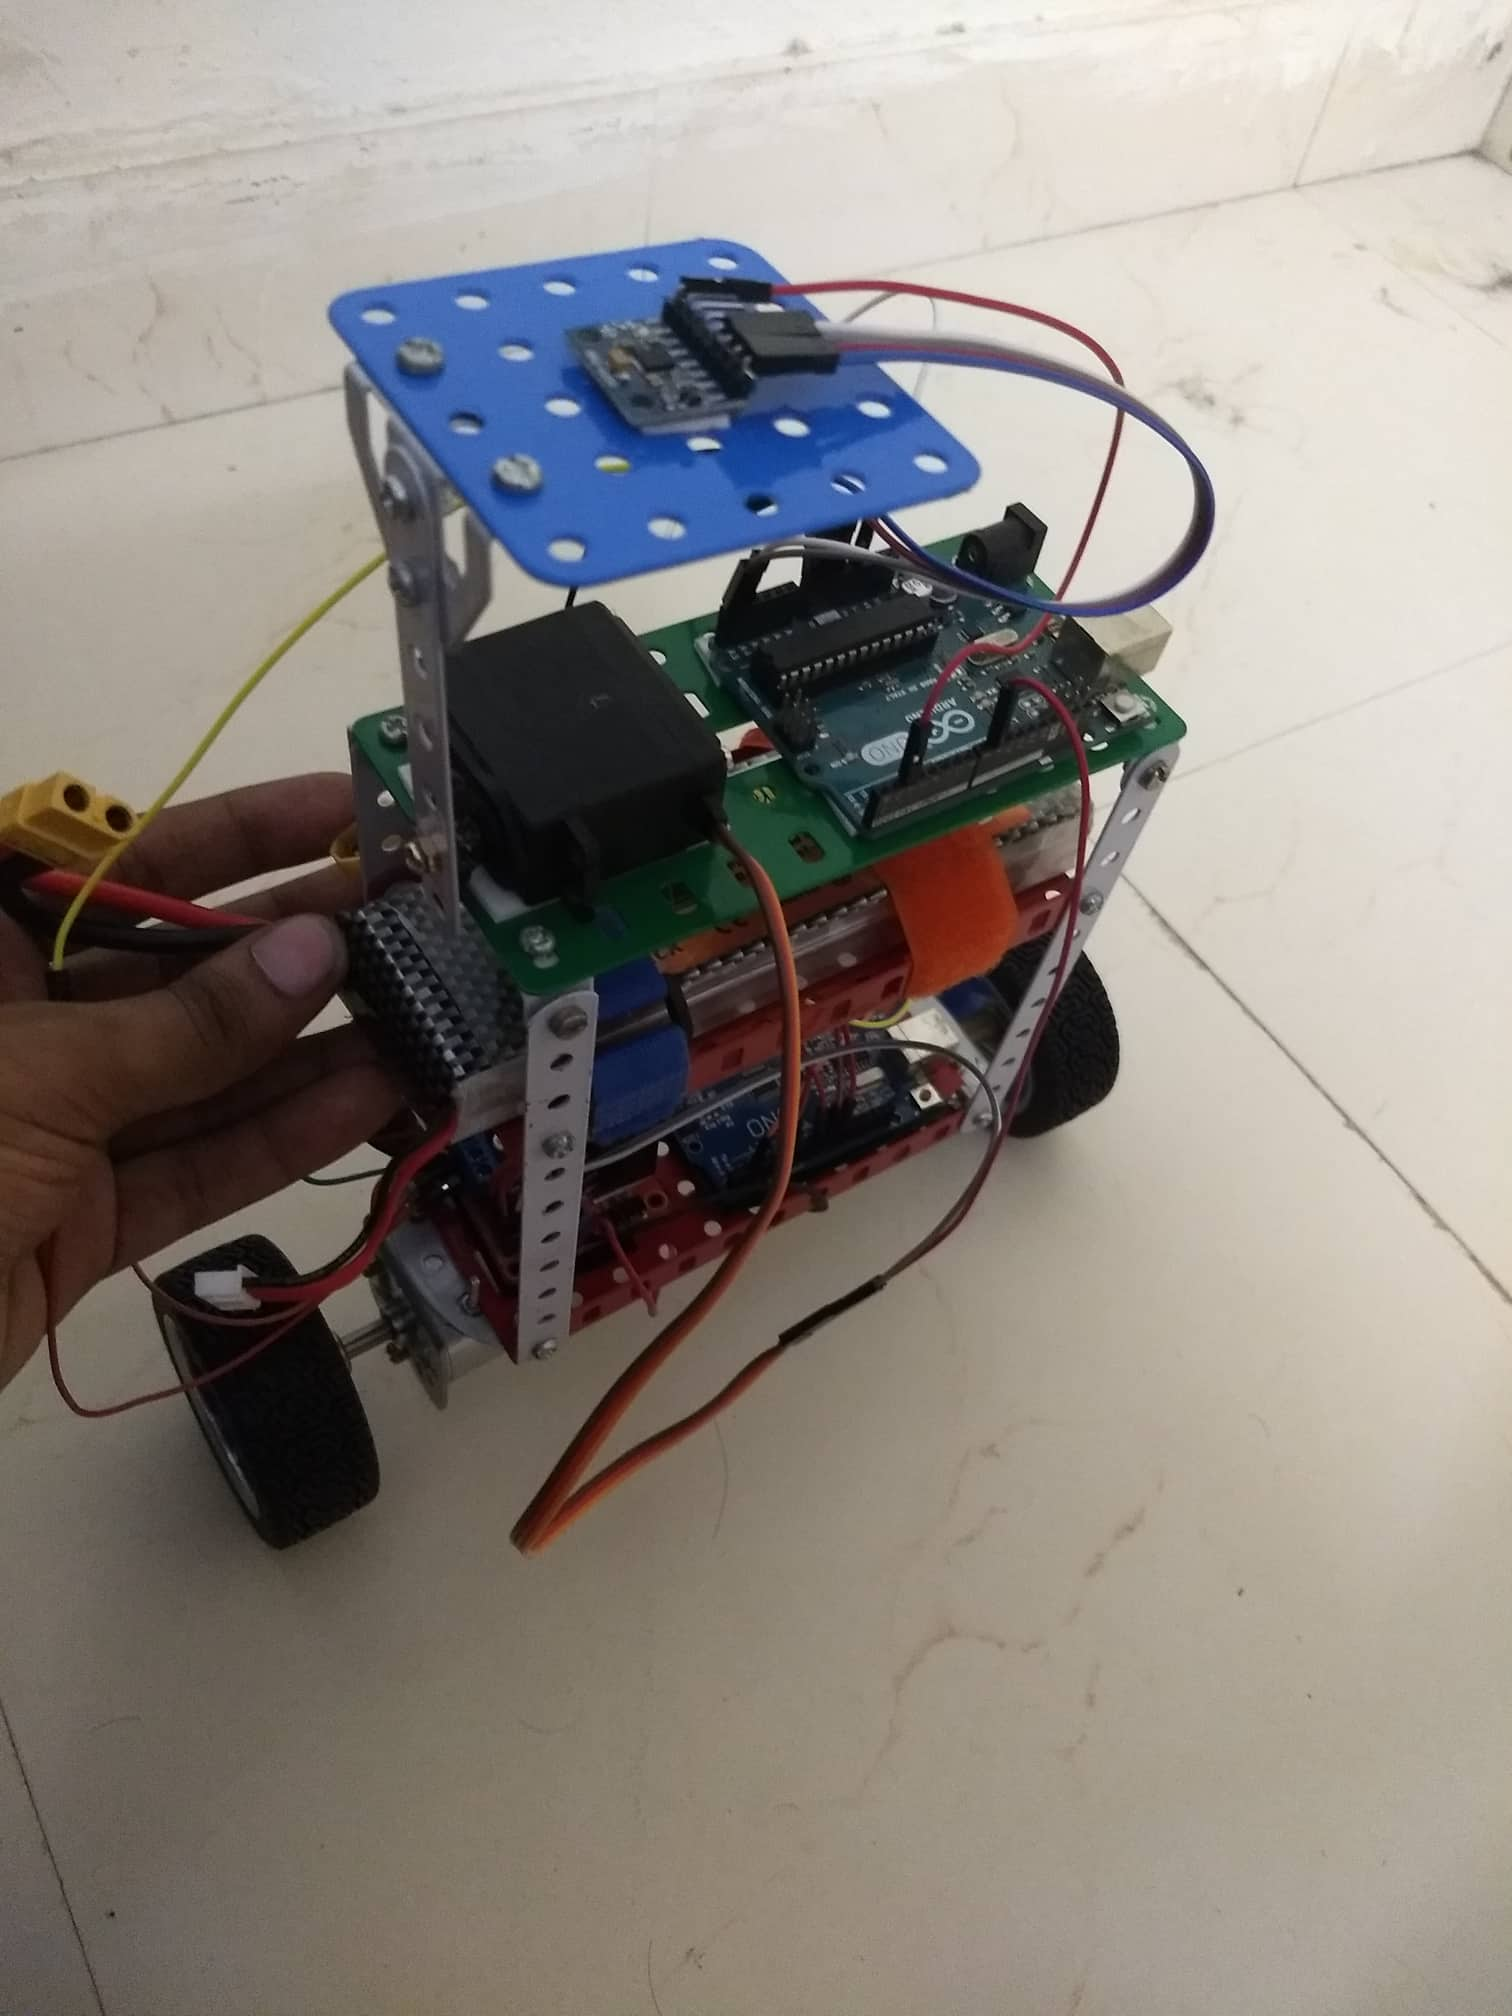
\includegraphics[width=.4\linewidth, scale = 2]{images/bot1}
  \caption{Arrangement of connections on platform}
  \label{fig:bot1}
\end{subfigure}%
\begin{subfigure}{.5\textwidth}
  \centering
  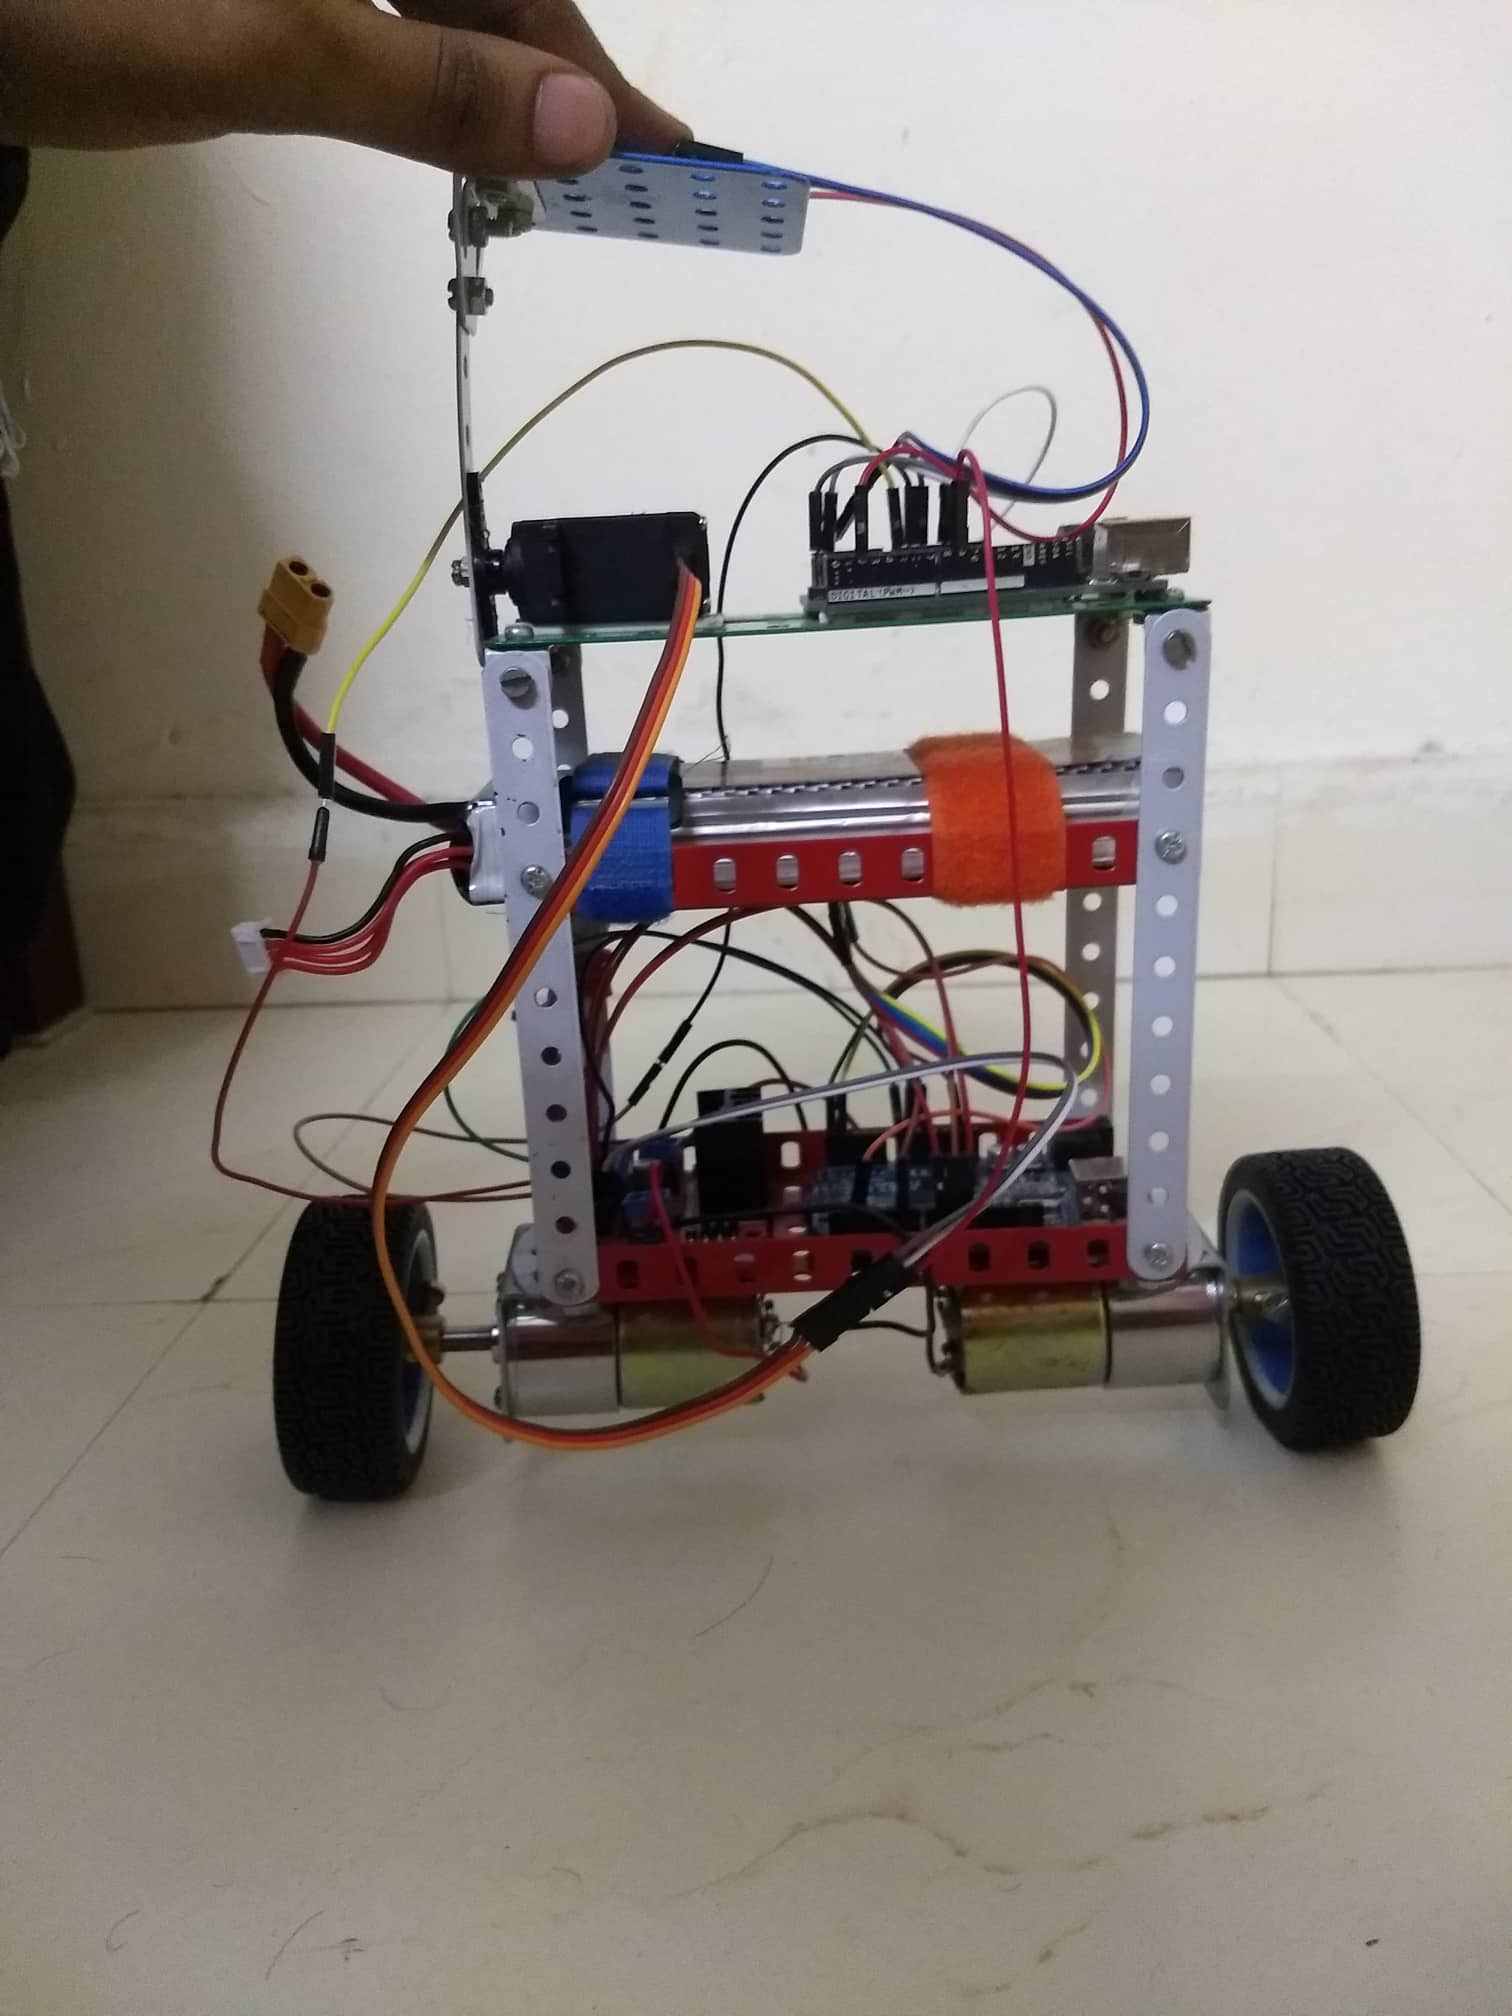
\includegraphics[width=.4\linewidth, scale = 2]{images/bot4}
  \caption{Arrangement of complete bot connections}
  \label{fig:bot2}
\end{subfigure}
\caption{Figure showing the arangement of connections for bot and platform}
\label{fig:combination}
\end{figure}

In figure \ref{fig:combination}, we see the manner in which the prescribed connections are arranged. For the self-balancing table, the arduino is stuck on the top layer of the chassis and the MPU6050 is fixed on top of the platform. \newline
For the self balancing bot, we see from figure \ref{fig:bot2} that the L298N motor driver and the arduino are pasted in the bottom layer of the chassis. The MPU6050 is fixed to the bottom side of the second layer and the battery is placed on the second layer of the chassis.
